\documentclass[captions=tableheading]{scrartcl}

\usepackage{amsmath}
\usepackage{amssymb}
\usepackage[utf8]{inputenc}
\usepackage[T1]{fontenc}
\usepackage{lmodern}
\usepackage{ngerman}
\usepackage{geometry}
\usepackage{graphicx}
\usepackage{wrapfig}
\usepackage{caption}
\usepackage{wasysym}
\usepackage[separate-uncertainty=true]{siunitx}
\usepackage{picinpar}
\usepackage{tikz}
\usepackage{float}
\usepackage{booktabs}

\renewcommand{\figurename}{Abb.}
\usepackage[
	colorlinks=true,
	urlcolor=blue,
	linkcolor=black
]{hyperref}


%Hier Titel und so
\newcommand{\versuchnummer}{V61} 
\newcommand{\versuchname}{Der He-Ne-Laser} 
\newcommand{\versuchdatum}{24.10.2016} 


\title{Versuch \versuchnummer\\ \versuchname}
\subtitle{Physikalisches Fortgeschrittenenpraktikum}
\author{Robert Rauter und Björn Lindhauer}
\date{\versuchdatum} 
\begin{document}
\begin{titlepage}
{\large \versuchdatum}
\vspace{7cm}
\begin{center}
\textbf{\huge Versuch \versuchnummer}\\\vspace{0.5cm}
\textbf{\huge \versuchname}\\
\vspace{0.2cm}
\textbf{ Physikalisches Fortgeschrittenenpraktikum}\\
\vspace{9cm}

{\Large Robert Rauter \ \ \hspace{1.5cm} und \hspace{1.5cm} Björn Lindhauer}\\
{ \url{robert.rauter@tu-dortmund.de} \ \ \hspace{2cm} \url{bjoern.lindhauer@tu-dortmund.de}}
\end{center}
\end{titlepage}
\section{Einleitung}
In diesem Versuch soll ein He-Ne-Laser auf charakteristische Eigenschaften untersucht werden. Dazu werden die Wellenlänge des Lasers, die TEM$_{00}$- und die TEM$_{01}$-Mode und die Polarisation des Lasers vermessen. Zudem wird die Stabilitätsbedingung des Resonators überprüft.
\section{Theoretische Grundlagen}
Der Begriff Laser steht für Light Amplification by Stimulated Emission of Radiation und beschreibt ein Gerät, welches monochromatisches Licht mit hoher Intensität und Kohärenz emittiert.

Ein Laser besteht aus drei grundlegenden Komponenten. Zum einem das aktive Medium, welches das Strahlungsspektrum eines Lasers bestimmt.
Ein weiterer Bestandteil des Lasers ist die Pumpquelle, die eine Besetzungsinversion durch stimulierte Emmision erzeugt. 
Schlussendlich gibt es noch den Resonator, der Licht durch optische Rückkopplung durch das aktive Medium leitet, sodass ein selbsterregter Oszillator entsteht.

Die genaue Funktionsweise eines Lasers lässt sich am einfachsten durch ein zwei Niveau System verstehen. 
Dabei sei das energetisch günstigere Niveau der Grundzustand mit der Besetzungszahl $n_1$ und das andere Niveau der angeregte Zustand mit der Besetzungszahl $n_2$, so gibt es drei verschiedene Übergänge.

Bei der Absorption wird ein Photon mit passender Energie absorbiert und das Atom in einen angeregten Zuständ überführt. 
Ein angeregtes Atom kann spontan in den Grundzustand zurückkehren, wobei dabei ein Photon emittiert wird. Dies wird spontane Emission genannt.
Alternativ kann eine Emission auch durch Bestrahlung mit energetisch passenden Photonen induziert werden, was induzierte Emission genannt wird.
In Abbildung \ref{fig:schema_uebergaenge} werden diese Übergänge illustriert.
\begin{figure}[h]
 \centering
 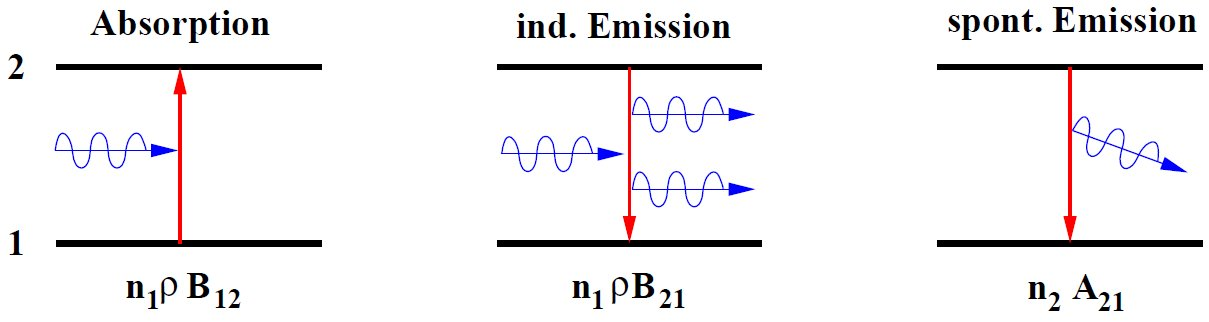
\includegraphics[width=12cm]{images/schema_uebergaenge.jpg}
  \caption{mögliche Übergänge in einem 2-Niveau-System [1]}
 \label{fig:schema_uebergaenge}
\end{figure}

Die Wechselwirkung zwischen der Energiedichte $\rho$ der Strahlungsfeldes und des Zwei-Niveau-Systems ist durch die Gleichung
\begin{align}
 \dot{N}_\text{A}   & =n_1 \rho\left(\nu \right)B_{12}  &\text{Absorption} \\
 \dot{N}_\text{IE}  & =n_2 \rho\left(\nu \right)B_{21}  &\text{induzierte Emission} \\
 \dot{N}_\text{SE}  & =n_2 A_{21}                       &\text{spontane Emission}
\end{align}
mit den Einsteinkoeffizienten $A_{21}$, $B_{12}$ und $B_{21}$, die Übergangswahrscheinlichkeiten zwischen den Zuständen beschreiben, gegeben.

Aus diesen Gleichungen lassen sich, unter der Bedingung, dass keine Verluste ($n_1+n_2=$const.) auftreten, die Ratengleichungen für die Besetzungszahlen
\begin{align}
 \frac{d n_1}{d t}&=-n_1B_{12}\rho+n_2B_{21}\rho+n_2A_{21}\rho \\
 \frac{d n_2}{d t}&=-n_2B_{21}\rho+n_1B_{12}\rho-n_2A_{21}\rho
\end{align}
herleiten.

Damit das Strahlungsfeld kohärent und dauerhaft verstärkt wird, muss die stimulierte Emission häufiger auftreten als die spontane Emission. 
Nun sind die Zustände nach Maxwell-Boltzmann besetzt, sodass der Grundzustand viel stärker besetzt ist als der angeregte Zustand und die spontane Emission dominiert.
Um dies zu ändern, muss der angeregte Zustand häufiger besetzt sein. Dies wird durch eine Besetzungsinversion realisiert. 
Damit die Besetzungsinversion dauerhaft ist, muss die ganze Zeit Energie in das aktive Medium zugeführt werden. Dies wird auch Pumpen genannt.

Da die Verstärkung exponentiell mit der Länge des Laufwegs des Lichts durch das aktive Medium steigt, wird der Laserstrahl durch einen optischen Resonator mehrfach durch das aktive Medium geleitet.

\begin{figure}[h]
 \centering
  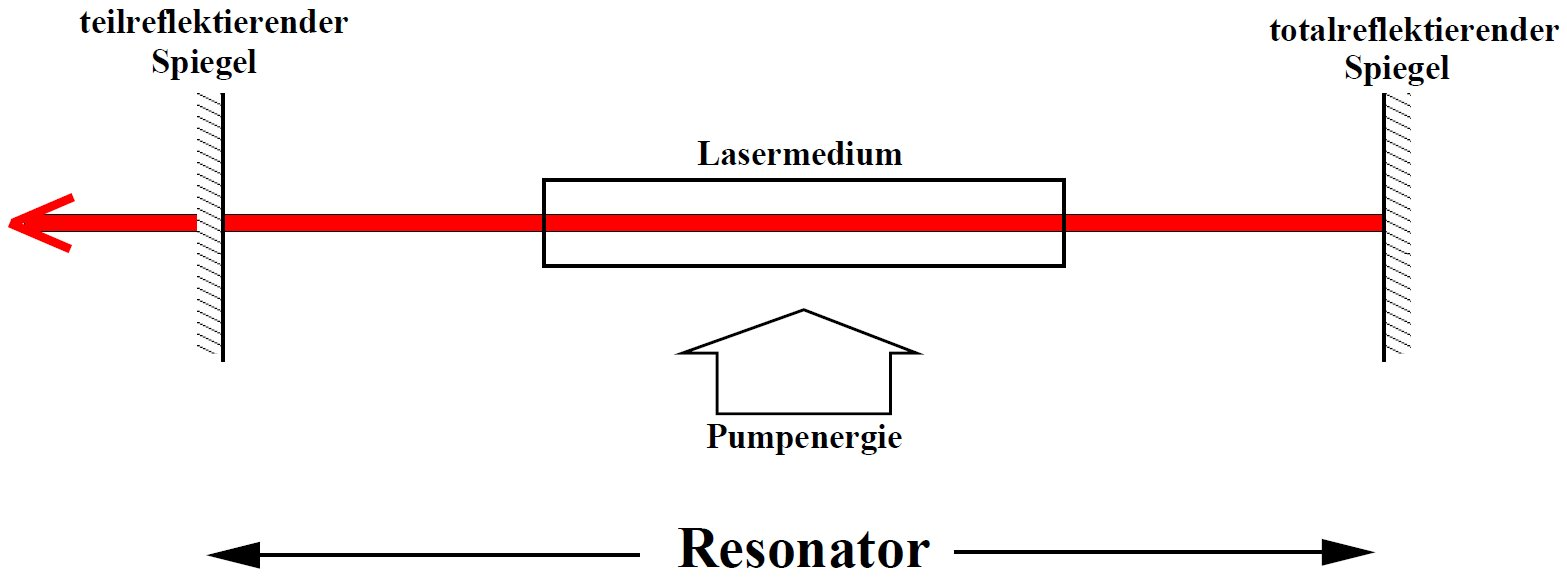
\includegraphics[width=12cm]{images/schema_resonator.jpg}
 \caption{Schematische Funktionsweise eines Lasers [1]} 
  \label{fig:schema_resonator}
\end{figure}

Wie in Abbildung \ref{fig:schema_resonator} dargestellt, besteht der optische Resonator aus zwei parallelen Spiegeln, von denen ein Spiegel teildurchlässig ist, um den Laserstrahl auszukoppeln.
Die Spiegel können dabei entweder nur planparallel oder nur sphärisch oder eine Kombination dieser beiden Typen sein.
Es sollten jedoch die Verluste durch die Spiegel geringer sein als die Verstärkung durch die angeregte Emission, damit ein angetriebener Oszillator entsteht.
Um eine charakteristische Grö"se für diese optische Stabilität zu erhalten, wird der Resonatorparameter
\begin{align}
 g_i := 1- \frac{L}{r_i}
\end{align}
mit der Länge $L$ des Resonators und der Krümmungsradius $r_i$ des Spiegels eingeführt.
Die optische Stabilität ist dann für
\begin{align}
0 \le g_1 \cdot g_2 \le 1 
\label{eq:stabilitaet}
\end{align}
gegeben.

Da die Resonatorlänge $L$ viel grö"ser als die Wellenlänge $\lambda$ sein soll, erfüllen viele Frequenzen die Resonzbedingungen für stehende Wellen. 
Diese $q$ Wellenlängen werden als longitudinale Mode bezeichnet. Es können auch transversalen Moden durch z.B. Spiegelunebenheiten oder Verkippungen entstehen.
In Anlehnung an einen Hohlleiter werden diese Moden $\text{TEM}_{lpq}$ genannt, wobei $l$ und $p$ die Knoten in x- und y- Richtung sind und als transversale Modenzahl bezeichnet werden.
Dabei ist $q$ die longitudinale Modenzahl und wird oft weg gelassen, da sie für die skalare Feldverteilung irrelevant ist.  

Die Feldverteilungen für einen konfokalen Resonator mit runden Spiegeln ist durch
\begin{align*}
 E_{lpq} \propto &\cos \left(l \phi \right) \frac{4\rho^ 2}{\left(1+Z^2 \right)^{0.5\cdot \left(1+l\right)}}L_{q}^{p}\left( \frac{4\rho^2}{1+Z^2} \right)\exp \left(-\frac{\rho^2}{1+Z^2}\right) \\
&\cdot\exp \left\{-i \left[ \frac{\left(1+Z \right)\pi R}{\lambda} + \frac{\rho^2Z}{1+Z^2} - \left(l+2p+1\right)\left(\frac{\pi}{2}-\arctan \left(\frac{1-Z}{1+Z}\right) \right) \right] \right\}
\end{align*}
\begin{align*}
\text{mit } \rho= \sqrt{\frac{2\pi}{R\lambda}} \text{ und } Z=\frac{2z}{R}
\end{align*}
approximativ gegeben. Dabei ist $L^{q}_{p}\left(u\right) $ das dazugehörige Laguerre-Polynom.

Aus dieser Feldverteilung lässt sich die Intensitätsverteilung bestimmen. Die Intensitätsverteilung der $\text{TEM}_{00}$ Mode, die Mode mit der höchsten Symmetrie und den geringsten Verlusten, ist durch die Gau"sverteilung
\begin{align}
 I\left(r\right)=I_0\exp \left(-\frac{2r^2}{\omega^2}\right)
 \label{eq:tem00}
\end{align}
mit der Maximalintensität $I_0$ gegeben. Der Strahlradius $\omega$ ist durch den Abstand $z$ von der minimalen Strahltaille $\omega_0$ und der Strahldivergenz 
\begin{align}
 \theta = \frac{\lambda}{\pi}\omega_0
\end{align}
gegeben. Er lässt sich durch
\begin{align}
 \omega\left(z\right)=\omega_0\sqrt{1+\left(\frac{\theta z}{\omega_0}\right)}
\end{align}
bestimmen. 

\section{Aufbau}
Für den HeNe-Laser wird ein Helium-Neon-Gemisch im Verhältnis 5:1 verwendet. Das Gasgemisch befindet sich bei einem Druck von ca. 1 Torr in einem zylindrischen Glasgefä"s. Die Neon-Atome dienen als aktives Medium, die Heliumatome als Pumpquelle. Über Stö"se wird die Energie an die Neon-Atome weitergegeben, welche in metastabile Zustände übergehen und Besetzungsinversion erzeugt. \\
Das Helium wird mithilfe von Elektroden-Entladungen gepumpt. Dominant bei diesem Laser ist die Wellenlänge $\lambda=\SI{632.8}{\nano\metre}$.\\
Zur möglichst verlustfreien Durchleitung des Laserlichts sind beide Enden des zylindrischen Glasgefä"ses mit Brewsterfenstern, die im Brewster-Winkel zur optischen Achse stehen, abgeschlossen, welche auch der Einstellung einer wohldefinierten Polarisationsrichtung dienen. Der Brewsterwinkel ist dabei der Winkel, unter welchem nur das senkrecht zur Einfallsebene polarisierte Licht reflektiert wird.\\
Ein bereits längs der optischen Achse ausgerichteter Justierlaser befindet sich ebenfalls auf der optischen Schiene, dieser kann zur Justage beim Aufbau des Resonators verwendet werden. Es stehen verschieden Spiegel, Gitter, Linsen und Photodioden zur Vermessung der Eigenschaften des Lasers zur Verfügung. 

\section{Durchführung}

\subsection{Bestimmung der Wellenlänge}
Zu Bestimmung der Wellenlänge wird ein Gitter mit Gitterkonstante g=100$\frac{1}{\si{\milli\metre}}$ in den Strahlgang gestellt und das Interferenzbild vermessen. Daraus wird die Wellenlänge des Lasers bestimmt.

\subsection{Vermessung der TEM-Moden}
Zur Vermessung der TEM$_{00}$-Mode wird der Laserstrahl mit einer Linse aufgeweitet und mithilfe einer verschiebbaren Photodiode und des Picoamperemeters ausgemessen. \\
Zur Vermessung der TEM$_{01}$-Mode wird ein dünner Wolframdraht in den Strahlgang gestellt, um so die TEM$_{00}$-Mode herauszufiltern. Auch diese Mode wird mithilfe der Photodiode und des Amperemeters vermessen.

\subsection{Polarisationsmessung}
Zur Ausmessung der Polarisation des Laserstrahls wird ein verstellbarer Polarisationsfilter in den Strahlengang gestellt und in $\ang{5}$-Schritten gedreht. Für jede Einstellung wird die Intensität aufgenommen.

\subsection{Überprüfung der Stabilitätsbedingung}
Mithilfe des angebrachten Justierlasers wird ein Resonator aufgebaut. Dazu werden zunächst ein konkaver Spiegel und ein planarer Spiegel verwendet, danach werden diese durch zwei konkave Spiegel ausgetauscht. Nach der korrekten Installation der Spiegel sowie der Justierung der Position des Spiegels wird die Laser-Tätigkeit erreicht. Danach wird die Resonatorlänge schrittweise erhöht, um die Stabilitätsbedingung zu überprüfen.

\section{Auswertung}

\subsection{Bestimmung der Wellenlänge des Lasers}
Zur Bestimmung der Wellenlänge des vom Laser emittierten Lichts wurden die Positionen von einem durch ein Gitter mit g=100$\frac{1}{\si{\milli\metre}}$ erzeugten Maxima aufgezeichnet. Diese Messwerte sind in Tabelle \ref{tab:maxima} dargestellt. \\
\begin{table}[H]
	\centering
		\captionof{table}{Distanz der einzelnen Maxima vom 0. Maximum}
		\label{tab:maxima}
		\begin{tabular}{r r}
			\toprule
			n & r [cm] \\
			\midrule
			-5 & 45.5 \\
			-4 & 36.1 \\
			-3 & 26.9 \\
			-2 & 17.8 \\
			-1 & 8.7 \\
			1 & 9.1 \\
			2 & 18.5 \\
			3 & 28.5 \\
			4 & 37.4 \\
			5 & 48.1 \\
			\bottomrule
		\end{tabular}
\end{table}
Die Wellenlänge ergibt sich dann aus der Formel für die Beugung am Gitter aus
\begin{align}
\lambda = \frac{\sin\left(\arctan\left( \frac{d}{L}\right) \right) }{ng}\quad.
\end{align}
Nach Mittlung über alle berechneten Wellenlängen ergibt sich die experimentell bestimmte Wellenlänge zu
\begin{align*}
\lambda = (636.42 \pm 43.44)\si{\nano\metre}\quad.
\end{align*}

\subsection{Ausmessung der TEM$_{00}$-Mode}
Für die Vermessung der TEM$_{00}$-Mode wurden Werte für den Photostrom $I$ in Abhängigkeit von der Position d der Photodiode aufgenommen, diese Werte sind in Tabelle \ref{tab:tem00} dargestellt.
\begin{table}
	\centering
	\captionof{table}{Werte für den Photostrom I in Abhängigkeit von der Position d der Photodiode}
	\label{tab:tem00}
	\begin{tabular}{c c c c}
		\toprule
				 d [mm] & I [$\mu$A] & d [mm] & I [$\mu$A]\\
		\midrule
				15	&	0	&	-1	&	0,076	\\
				14	&	0	&	-2	&	0,07	\\
				13	&	0	&	-3	&	0,066	\\
				12	&	0	&	-4	&	0,078	\\
				11	&	0	&	-5	&	0,082	\\
				10	&	0,004	&	-6	&	0,078	\\
				9	&	0,004	&	-7	&	0,058	\\
				8	&	0,005	&	-8	&	0,06	\\
				7	&	0,007	&	-9	&	0,039	\\
				6	&	0,01	&	-10	&	0,023	\\
				5	&	0,023	&	-11	&	0,023	\\
				4	&	0,03	&	-12	&	0,016	\\
				3	&	0,064	&	-13	&	0,004	\\
				2	&	0,074	&	-14	&	0,007	\\
				1	&	0,096	&	-15	&	0,006	\\
				0	&	0,09	&		&		\\
		\bottomrule
	\end{tabular}
\end{table}
Aus Gleichung \ref{eq:tem00} folgt, dass der Verlauf der TEM$_{00}$-Mode die Form einer Gau"s-Funktion besitzen muss, mit $r_0$ der Nullposition der Photodiode und $\omega$ dem Strahlradius. \\
Ein nicht-linearer Fit mithilfe von \textit{python} ergibt die Fit-Parameter
\begin{align*}
I_0=& (0.088 \pm 0.004) \si{\mu\ampere}\\
r_0=& (-2.362 \pm 0.276) \si{\milli\metre}\\
\omega=&  (10.230  \pm 0.554) \si{\milli\metre}\quad.
\end{align*}
Die angepasste Theoriekurve und die Messwerte sind in Abbildung \ref{fig:tem00} dargestellt.
\begin{center}
	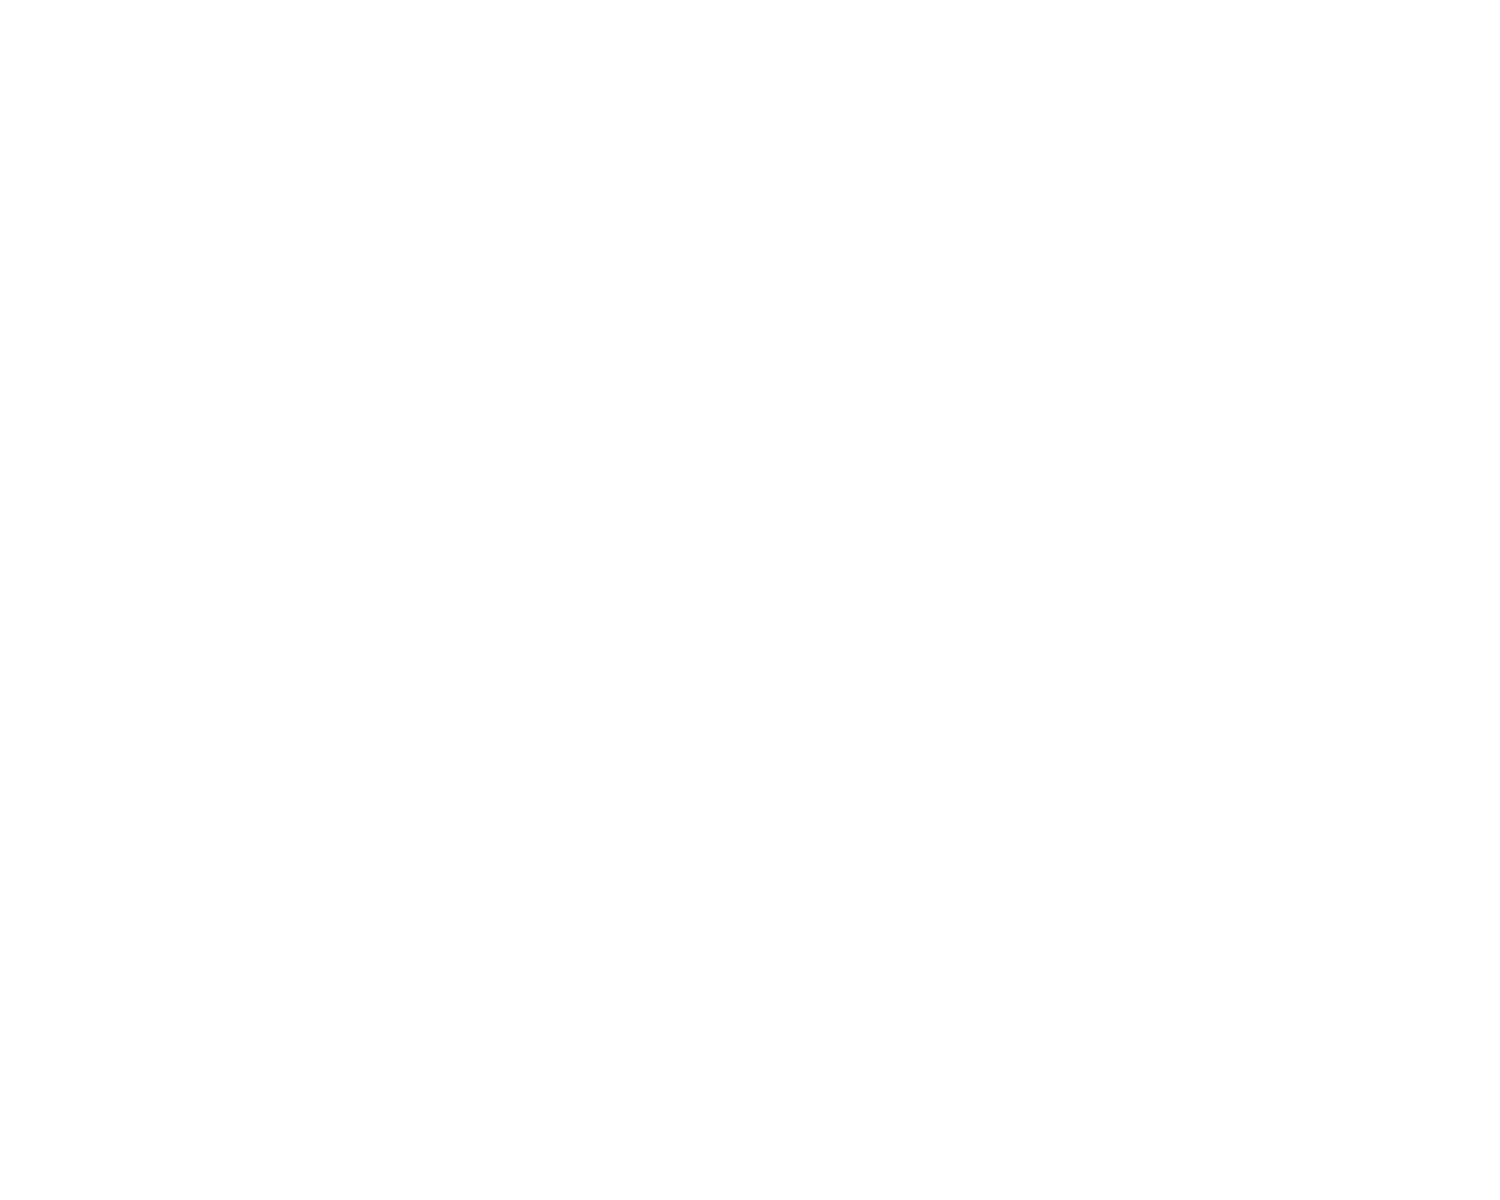
\includegraphics[width=10cm]{images/tem00.pdf}
	\captionof{figure}{Messwerte für den Photostrom I in Abhängigkeit von der Diodenposition und angepasste Theoriekurve}
	\label{fig:tem00}
\end{center}
\subsection{Polarisationsmessung}
Der in Abhängigkeit von der Winkeleinstellung des Polarisationsfilters gemessene Fotostrom ist in Tabelle \ref{tab:polarisation} dargestellt.
\begin{table}
	\centering
	\captionof{table}{Werte für den Photostrom I in Abhängigkeit von dem eingestellten Winkel $\phi$}
	\label{tab:polarisation}
	\begin{tabular}{r r r r}
	\toprule $\phi$ [$^{\circ}$] & I [$\mu$A] & $\phi$ [$^{\circ}$] & I [$\mu$A]\\
	\midrule 0	&	0.53	&	95	&	1.2	\\
		   5	&	0.4	&	100	&	1.39	\\
	   	  10	&	0.32	&	105	&	1.6	\\
		  15	&	0.25	&	110	&	1.6	\\
	   	  20	&	0.14	&	115	&	1.7	\\
		  25	&	0.06	&	120	&	1.8	\\
		  30	&	0.02	&	125	&	1.7	\\
		  35	&	0.01	&	130	&	1.9	\\
		  40	&	0.03	&	135	&	1.9	\\
		  45	&	0.07	&	140	&	1.8	\\
		  50	&	0.13	&	145	&	1.7	\\
		  55	&	0.21	&	150	&	1.5	\\
		  60	&	0.36	&	155	&	1.5	\\
		  65	&	0.46	&	160	&	1.3	\\
		  70	&	0.6	&	165	&	1	\\
		  75	&	0.71	&	170	&	0.8	\\
		  80	&	0.9	&	175	&	0.8	\\
		  85	&	0.98	&	180	&	0.65	\\
		  90	&	1.27	&		&		\\				
	\bottomrule
		\end{tabular}
\end{table}
Die Intensität in Abhängigkeit vom eingestellten Winkel des Polarisationsfilters ist durch 
\begin{align}
T(\phi)=I_0\cos\left(\phi+\delta\right)^2
\end{align}
gegeben. \\
Die Fit-Parameter ergeben sich zu
\begin{align*}
I_0&=(1.815 \pm 0.019)\si{\mu\ampere} \\
\delta&=(0.944 \pm 0.009)\quad.
\end{align*}
Messwerte und Fit sind in Abbildung \ref{fig:pol} dargestellt. Es ist deutlich sichtbar, dass die Intensität für $\phi=\ang{125.9}$ maximal wird.
\begin{center}
 	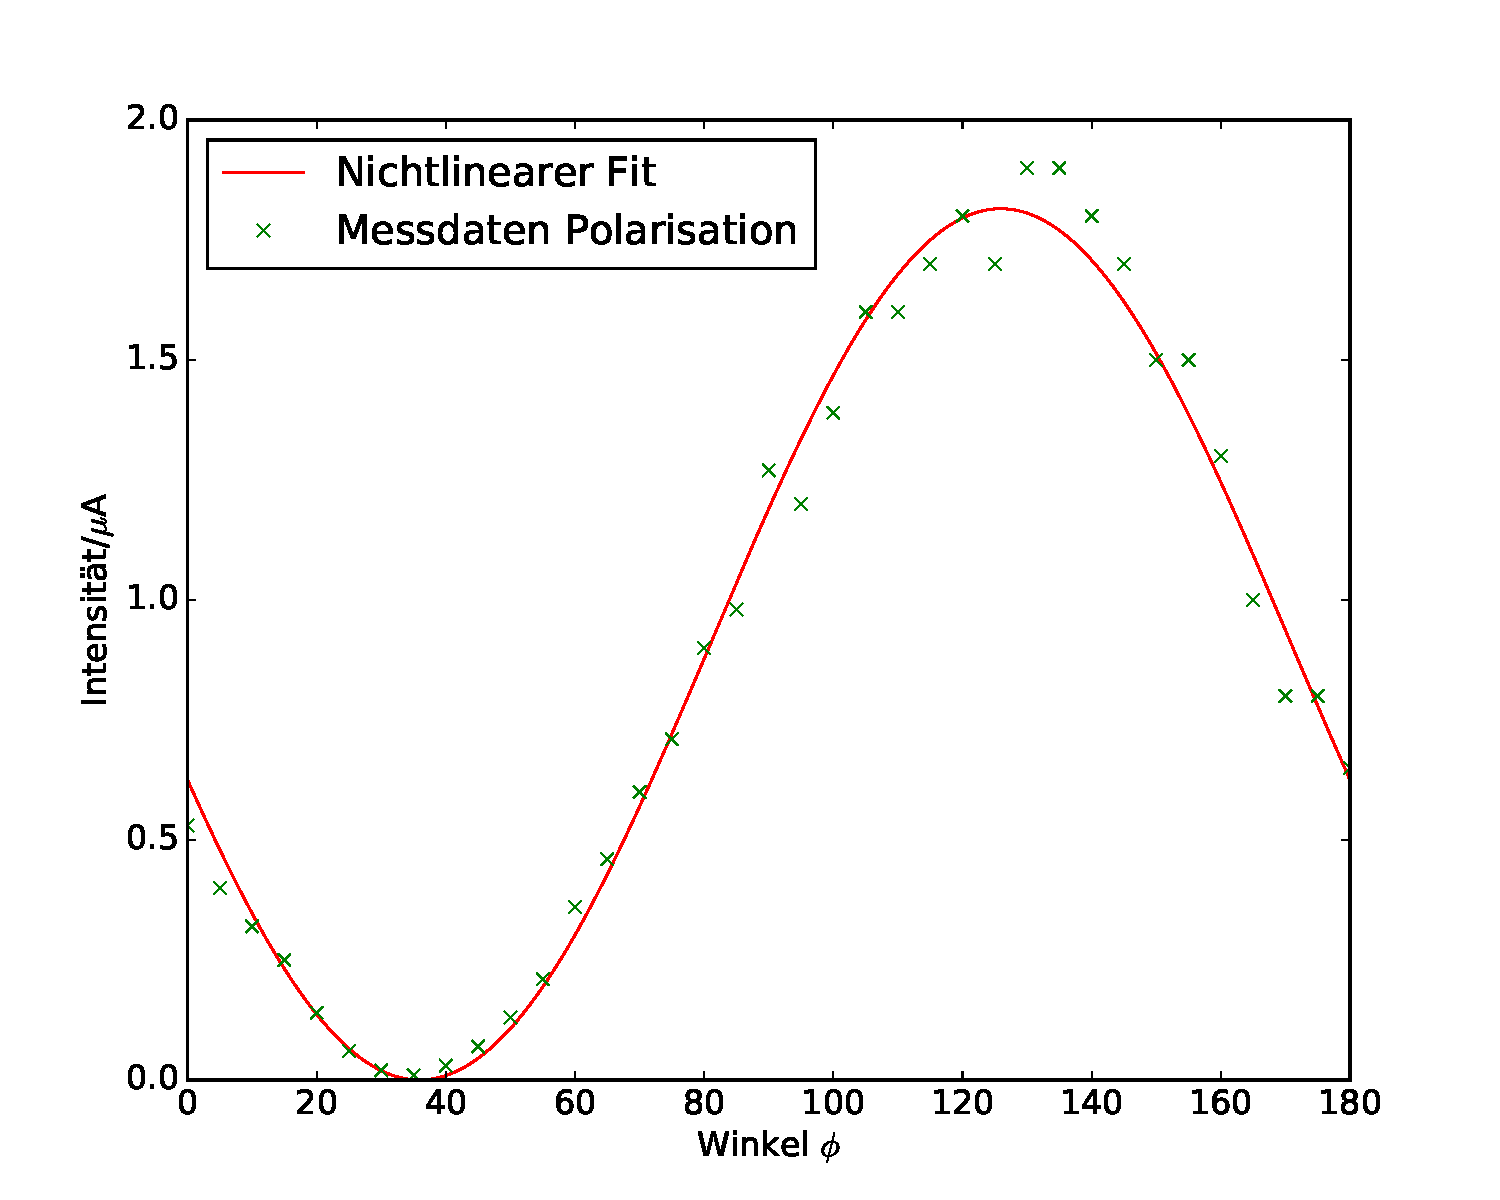
\includegraphics[width=10cm]{images/polarisation.pdf}
 	\captionof{figure}{Messwerte für den Photostrom I in Abhängigkeit von des eigestellten Winkels des Polarisationsfilters und angepasste Theoriekurve}
 	\label{fig:pol}
\end{center}

\subsection{Überprüfung der Stabilitätsbedingung}
Zur Untersuchung der Stabilität des Lasers wurden zwei Konfigurationen von Spiegeln verwendet. Es wurden Spiegel mit Krümmungsradien r$_1=1\si{\meter}$ und r$_2=1.4\si{\meter}$ sowie r$_1=1\si{\meter}$ und r$_2=\infty\si{\meter}$, d.h. einem planaren Spiegel, verwendet. \\
Gemä"s der Stabilitätsbedingung aus Gleichung \ref{eq:stabilitaet} wurden dann Graphen erstellt, an welchen die maximale Distanz L abzulesen ist. Diese sind in Abbildung \ref{fig:stab} zu sehen. \\
\begin{center}
	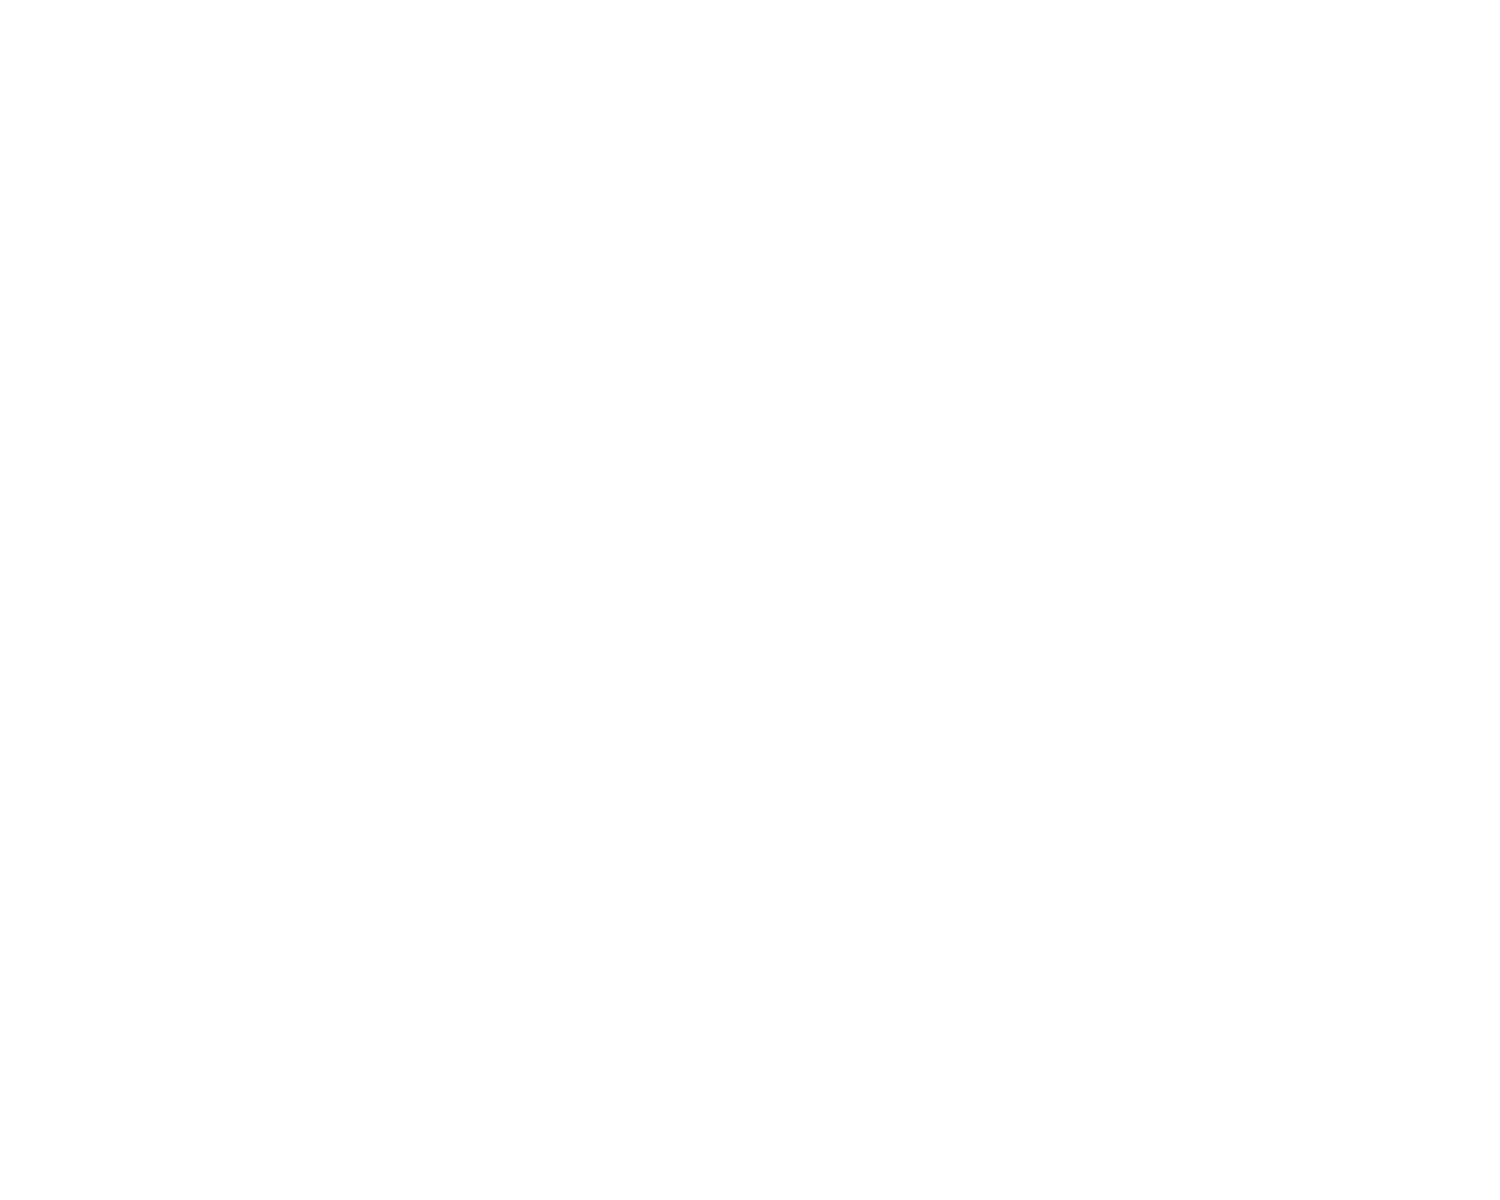
\includegraphics[width=10cm]{images/vorbereitung.pdf}
	\captionof{figure}{Stabilitätskurven des Lasers bei verschiedenen Linsenkonfigurationen}
	\label{fig:stab}
\end{center}
Aus der Abbildung können die beiden maximalen Längen L$_1=1.4\si{\meter}$ und L$_2=1\si{\metre}$ abgelesen werden. Im Experiment konnte nur die Kombination eines Spiegels mit Krümmungsradius r$=1.4\si{\metre}$ und eines planaren Spiegels verwendet werden. Die maximal erreichbare Resonatorlänge betrug dabei L$_{\text{max}}=1.34\si{\meter}$.

\section{Diskussion}

\subsection{Bestimmung der Wellenlänge}
Die experimentell bestimmte Wellenlänge von $\lambda = \SI{636.42(4344)}{\nano\metre}$ stimmt gut mit der in der Anleitung angegebenen Wellenlänge von $\lambda = \SI{632.8}{\nano\metre}$ überein. Der Fehler ist auf die begrenzte Ablesegenauigkeit zurückzuführen, diese betrug $\Delta d=\SI{0.3}{\centi\metre}$.

\subsection{Vermessung der TEM-Moden}
Aufgrund der sehr geringen Leistung des He-Ne-Lasers konnten weder die longitudinalen Moden noch die TEM$_{01}$-Mode vermessen werden. Mögliche Gründe dafür sind Verunreinigungen in der Apparatur und eine ungenaue Justierung. \\
Die gemessenen Messdaten spiegeln in Grundzügen den theoretischen Verlauf der TEM$_{00}$-Mode wieder. Abweichungen können wie bereits erwähnt durch ungenaue Justierung und Verunreinigungen erklärt werden. \\
Für die fit-Parameter haben sich  $I_0= (0.088 \pm 0.004) \si{\mu\ampere},\,r_0= (-2.362 \pm 0.276) \si{\milli\metre},\,\omega=  (10.230  \pm 0.554) \si{\milli\metre}$ ergeben. Die Unsicherheiten der Parameter liegen für $I_0$ und $r_0$ in der zweiten siginifikanten Stelle und für $\omega$ in der dritten signifikanten Stelle. Damit sind die Parameter mit ausreichender Genauigkeit bestimmt.

\subsection{Polarisationsmessung}
Die aufgenommenen Messwerte folgen der von der Theorie vorhergesagten Cosinus-Form. Es ergaben sich leichte statistische Abweichungen, die jedoch kaum signifikant sind. Die Fit-Paramter lauten $I_0=(1.815 \pm 0.019)\si{\mu\ampere},\, \delta=(0.944 \pm 0.009)$. \\
Diese Übereinstimmung mit dem Malusschen Gesetz zeigt, dass die Resonatorspiegel kaum einen Einfluss auf die Polarisation des Lasers haben. \\
Das Maximum bei $\phi=\ang{125.9}$ zeigt, dass der Laser in dieser Richtung polarisiert ist.

\subsection{Überprüfung der Stabilitätsbedingung}
Die theoretisch mögliche Resonatorlänge betrug $\SI{1.4}{\metre}$, dies wurde mit einer experimentell erreichten Resonatorlänge von $\SI{1.34}{\metre}$ nahezu erreicht. Die kleine Abweichung kann durch ein imperfektes Gesamtsystem, d.h. zum Beispiel leichte Erschütterung des Tisches, erklärt werden.

\section{Quellen}
{[1]} Physikalisches Praktikum, TU Dortmund: \\
Versuchsanleitung zu Versuch 61: \\
http://129.217.
224.2/HOMEPAGE/PHYSIKER/MASTER/SKRIPT/V61.pdf (letzte Version vom 16.11.2016, 09:45)\\

\end{document}